\documentclass[11pt,compress,t,notes=noshow, xcolor=table]{beamer}


\input{../../style/preamble}
\input{../../latex-math/basic-math}
\input{../../latex-math/basic-ml}


\newcommand{\titlefigure}{figure_man/linesearch.png}
\newcommand{\learninggoals}{
\item Iterative Descent / Line Search
\item Descent directions
\item GD
\item ERM with GD
\item Pseudoresiduals
}


%\usepackage{animate} % only use if you want the animation for Taylor2D

\title{Optimization in Machine Learning}
%\author{Bernd Bischl}
\date{}

\begin{document}

\lecturechapter{First order methods: Gradient descent}
\lecture{Optimization in Machine Learning}
\sloppy

\begin{vbframe}{Iterative Descent}

	Let $f$ be the height of a mountain depending on the geographic coordinates $(x_1, x_2)$
	\vspace*{-0.1cm}
	$$
	f: \R^2 \to \R, \q     uad f(x_1, x_2) = y.
	$$
	
	\textbf{Goal}: Reach the valley

	$$
	\argmin f(\xv)
	$$
	
	\textbf{Central idea}: Repeat
	\vspace*{-0.15cm}
	\begin{columns}
		\begin{column}{0.58\textwidth}
			\begin{enumerate}
				\item At current location $\xv \in \R^d$ search for \textbf{descent direction} $\mathbf{d}$ 
			  	\item Move along $\mathbf{d}$ until $f$ sufficiently reduced (\textbf{step size control}) and update location
			\end{enumerate}
		\end{column}
		\begin{column}{0.4\textwidth}
			\begin{center}
			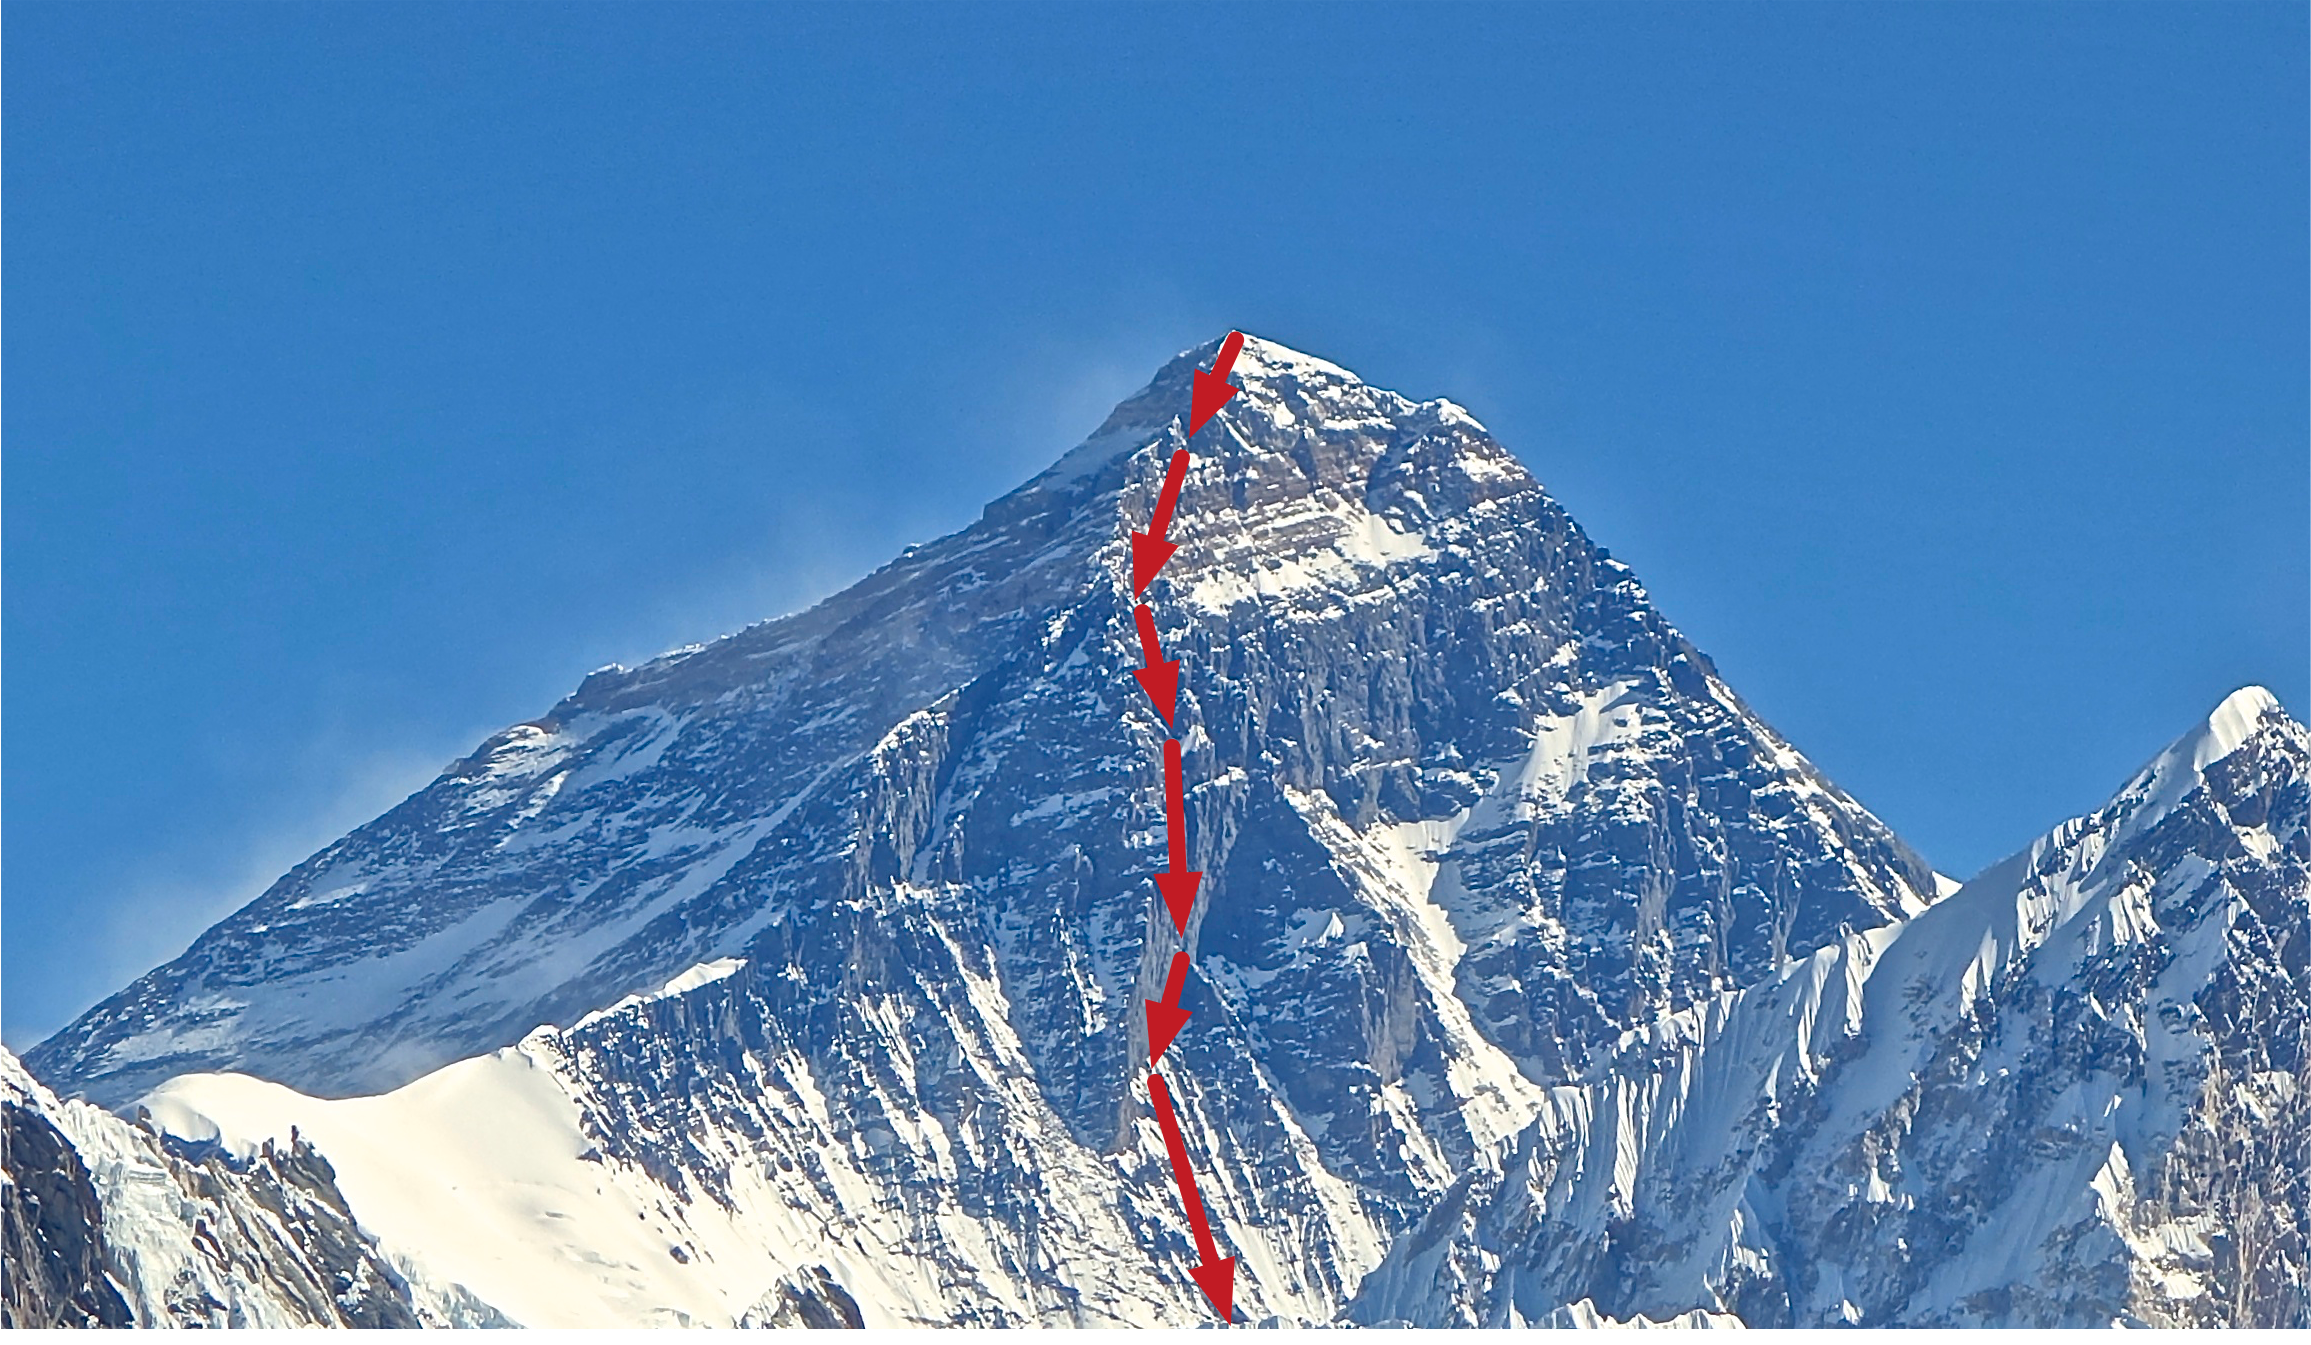
\includegraphics[width = 0.8\textwidth]{figure_man/linesearch.png}
			\hspace{2cm} \begin{footnotesize} "Walking down the hill, towards the valley." \end{footnotesize}\\
			\end{center}
		\end{column}
	\end{columns}
	
\end{vbframe}

\begin{vbframe}{Iterative Descent}

	Let $f: \R^d \to \R$ continuously differentiable.
	
	\lz
	
	\textbf{Definition:} $\mathbf{d}\in \R^d /\ \{\mathbf{0}\}$ is a \textbf{descent direction} in $\xv$ if
	$$
	D_d f(\xv) = \nabla f(\xv) ^T \mathbf{d} < 0 \text{ (neg. directional derivative)}
	$$

	\begin{figure}
		\includegraphics[width = 0.4\textwidth]{figure_man/descent_direction.pdf} \\
		\begin{footnotesize}
			Angle between $- \nabla \fx$ and $d$ must be $\in (90^{\circ}, 270^{\circ})$. 
		\end{footnotesize}
	\end{figure}

	% \framebreak 

	% \begin{figure}
	% 	\includegraphics[textwidth]{figure_man/branin_dirderiv.jpg} \\
	% 	\begin{footnotesize}
 %            Scaled directional derivatives in various directions as well as gradient and negative gradient.
 %            Colors indicate if ascending or descending.
	% 	\end{footnotesize}
	% \end{figure}

	\framebreak
	
	\begin{algorithm}[H]
	  \caption{Iterative Descent / Line search}
	  \begin{algorithmic}[1]
	  \State Starting point $\xv^{[0]} \in \R^d$
	  \While {Stopping criterion not met}
	    \State Calculate a descent direction $\mathbf{d}^{[t]}$ for current $\xv^{[t]}$
	    \State Find $\alpha^{[t]}$ s.t. $f(\xv^{[t + 1]}) < f(\xv^{[t]})$ for $\xv^{[t + 1]} = \xv^{[t]} + \alpha^{[t]} \mathbf{d}^{[t]}$
	   .
	    \State Update $\xv^{[t + 1]} = \xv^{[t]} + \alpha^{[t]} \mathbf{d}^{[t]}$
	  \EndWhile
	  \end{algorithmic}
	\end{algorithm}
	\vspace*{-0.2cm}
	\begin{tiny}
		NB: Terminology is sometimes ambiguous: ``line search'' can refer to Step 4 (selecting the step size that decreases $f(\xv)$) and can mean umbrella term for iterative descent algorithms. \par
	\end{tiny}

	\lz 

	Key questions: 
	\begin{itemize}
		\item How do choose $\mathbf{d}^{[t]}$ (now)
		\item How do choose $\alpha^{[t]}$ (later)
	\end{itemize}

\end{vbframe}

%%%

\begin{vbframe}{Gradient Descent}

	Properties of gradient: 

	\begin{itemize}
		\item $\nabla \fx$: direction of greatest increase
		\item $- \nabla \fx$: direction of greatest decrease
	\end{itemize}

	\vspace*{0.3cm}

	Using $\mathbf{d} = - \nabla \fx$ is called \textbf{gradient descent}. 

	\begin{center}
		\includegraphics[width = 0.8\textwidth]{figure_man/example-descent1.png} \\
		\begin{footnotesize}
			GD for $f(x_1, x_2) = - \sin(x_1) \cdot \frac{1}{2\pi} \exp\left( (x_2 - \pi / 2)^2 \right)$ with sensibly chosen step size $\alpha^{[t]}$. 
		\end{footnotesize}
	\end{center}


\end{vbframe}

\begin{vbframe}{GD and Multimodal functions}

Outcome will depend on start point. 

\begin{figure}
	\includegraphics[width=0.45\textwidth]{figure_man/gradient_descent_branin.pdf} \includegraphics[width=0.45\textwidth]{figure_man/gradient_descent_branin2.pdf}\\
	\vspace*{-0.3cm}
	\begin{footnotesize}
		$100$ iters of GD with const $\alpha = 10^{-4}$.
	\end{footnotesize}
\end{figure}

\end{vbframe}

%%%


\begin{vbframe}{Optimize LS linear regression with GD}

	\begin{footnotesize}

	Let $\D = \Dset$ and minimize 

	$$
		\risket = \sumin \left(\thetab^\top \xi - \yi\right)^2
	$$
	\textbf{NB: } For illustration, we use GD even though closed-form solution exists. GD-like (more adv.) approaches like this MIGHT make sense for large data, though.
	\end{footnotesize}
	
	\begin{footnotesize}
	\begin{eqnarray*}
	\textbf{Gradient: } && \nabla_{\thetab}\riske(\thetab) =  \frac{\partial \riske(\thetab)}{\partial
	\thetab} = - \sum_{i=1}^n 2 \cdot \left(y^{(i)} - \thetab^{\top} \xv^{(i)}\right) \xv^{(i)} \\
	% \textbf{GD Update: } && \thetatn \leftarrow \thetat + \alpha^{[t]} \sum_{i=1}^n 2 \cdot \left(y^{(i)} - \thetab^{[t]\top} \xv^{(i)}\right) \xv^{(i)}
	\end{eqnarray*}
	\end{footnotesize}

	% $\alpha^{[t]}$ also called \textbf{learning rate} in context of ERM.

	\vspace*{-0.5cm}

	\begin{center}
	\includegraphics[width=0.8\textwidth]{figure_man/gradient_descent_lm.pdf}
	\end{center}

\end{vbframe}

\begin{vbframe}{ERM for NN with GD}

Let $\D = \Dset$, with $y = x_1^2 + x_2^2$ and minimize 

\vspace*{-0.3cm}

$$
	\risket = \sumin \left(\fxt - \yi\right)^2
$$

\vspace*{-0.1cm}

where $\fxt$ is a neural network with 2 hidden layers (2 units each). 

\vspace*{-1.5cm}

\begin{figure}
	\includegraphics[width=0.6\textwidth]{figure_man/gradient_descent_NN_0.pdf}
\end{figure}

\framebreak 

After $10$ iters of GD: 

\begin{figure}
	\includegraphics[width=0.55\textwidth]{figure_man/gradient_descent_NN_10_surface.pdf} ~~ \includegraphics[width=0.4\textwidth]{figure_man/gradient_descent_NN_300_history.pdf}
\end{figure}

\framebreak 

After $100$ iters of GD: 

\begin{figure}
	\includegraphics[width=0.55\textwidth]{figure_man/gradient_descent_NN_100_surface.pdf} ~~ \includegraphics[width=0.4\textwidth]{figure_man/gradient_descent_NN_300_history.pdf}
\end{figure}

\framebreak 

After $300$ iters of GD (note the zig-zag-behavior after iter. 200):

\begin{figure}
	\includegraphics[width=0.55\textwidth]{figure_man/gradient_descent_NN_300_surface.pdf} ~~ \includegraphics[width=0.4\textwidth]{figure_man/gradient_descent_NN_300_history.pdf}
\end{figure}
\end{vbframe}

\begin{vbframe}{GD for ERM: Pseudoresiduals}

\begin{footnotesize}

Gradient for ERM problem: 

\vspace*{-0.5cm}

\begin{eqnarray*}
- \pd{\risket}{\thetab} &=& - \pd{\sumin \Lxyit}{\thetab}= - \sumin \underbrace{\pd{\Lxyi}{\fxi}}_{\text{pseudo residual } \tilde r^{(i)}(f)} \pd{\fxit}{\thetab}
\end{eqnarray*}

\vspace*{-0.5cm}

\begin{itemize}
	\item \textbf{pseudo residuals} tell us how to distort $\fxi$ to achieve greatest decrease of $\Lxyi$ (best pointwise update)
	\item $\pd{\fxit}{\thetab}$ tells us how to modify $\thetab$ accordingly and wiggle model output
	\item GD step sums up these modifications across all observations $i$
\end{itemize}

\begin{minipage}[b]{0.45\textwidth}
  \textbf{NB:} Pseudo-residuals 
  $\tilde{r}\left( f \right)$ 
  match usual residuals for L2 loss:
  \begin{align*}
  - \pd{\Lxy}{\fx} & = - \pd{0.5(y - \fx)^2}{\fx}\\ 
                   & = y - \fx
  \end{align*}
\end{minipage}%
\begin{minipage}[b]{0.05\textwidth}
   \phantom{foo}
\end{minipage}
\begin{minipage}[b]{0.45\textwidth}
  \includegraphics[width=0.9\textwidth]{figure_man/pseudo_residual_1.png}
  % Taken from lecture_sl, chapter advriskmin
\end{minipage}

\end{footnotesize}


\end{vbframe}


\endlecture
\end{document}

%%% 



%% 